\section{Discussion}
\subsection{Comparing Fitness vs Imitation Dynamics}
	\begin{figure}[h]
	      \centering
	      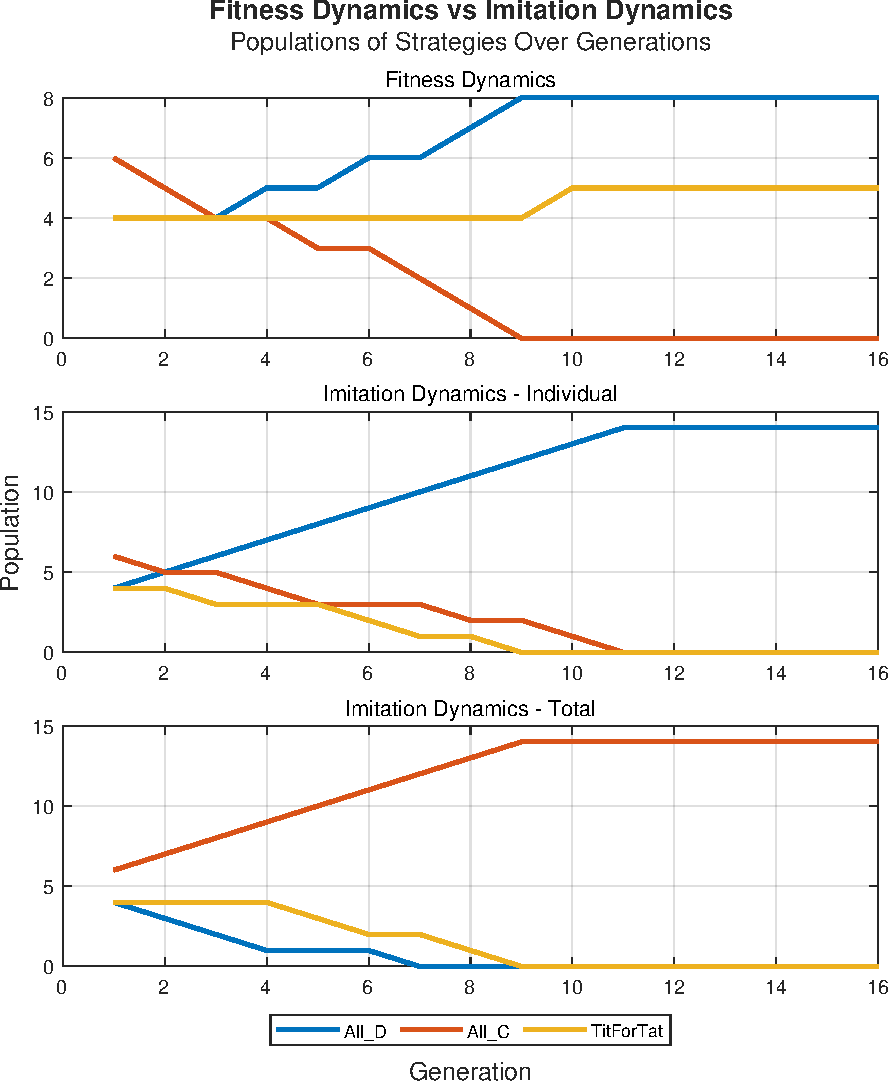
\includegraphics[width=0.9\textwidth]{Fitness Dynamics vs Imitation Dynamics.pdf}
	      \caption{Fitness Dynamics vs Imitation Dynamics $\begin{bmatrix}All\_D&All\_C&TitForTat\end{bmatrix}$ $POP0=\begin{bmatrix}4&6&4\end{bmatrix}$}
	      \label{fig:Fitness Dynamics vs Imitation Dynamics}
	\end{figure}
In Figure~\ref{fig:Fitness Dynamics vs Imitation Dynamics}, a comparison is made between the results of \texttt{TourSimFit}, \texttt{TourSimImi} with \texttt{mode = 'Individual'}, and \texttt{TourSimImi} with \texttt{mode = 'Total'} for the strategies 
\[
\begin{bmatrix} \text{All\_D} & \text{All\_C} & \text{TitForTat} \end{bmatrix}
\]
with initial population 
\[
POP0 = \begin{bmatrix} 4 & 6 & 4 \end{bmatrix}.
\]

We observe that the \texttt{Fitness} case resembles the \texttt{Individual} mode of the imitation dynamics. However, a key difference is noted: in the imitation dynamics, only one strategy survives. The \texttt{Total} mode exhibits a similar evolution to the \texttt{Individual} mode, but we observe that a different strategy survives—specifically, \texttt{All\_C}. This occurs because it has a higher initial population compared to the other strategies, and thus is better able to take advantage of the cooperative strategy \texttt{TitForTat} through the mechanism of the \texttt{Total} mode in identifying the best-performing strategy. This is obviously just an examplary simulation and there are way more comparisons to be made, which are left as a fun puzzle for the reader.

\subsection{Conclusions}
From the analysis of the Evolutionary Games we conclude the following:
\begin{enumerate}
\item The two dynamics offer different outlooks to the evolutionary aspect of the game, thus creating vastly different results.

\item Even for the same dynamics, minor changes like the ones in ``compensation'' mode or ``Individual'' vs ``Total'' the results can change drastically.

\item Important aspects to be considered for the results are the strategies used, the initial population, the payoff matrix, the game length and the population magnitude.
\end{enumerate}

Possible improvements of this toolbox include:

\begin{enumerate}
\item The inclusion of proper handling for random strategies. Currently it is impossible because of a fast but deterministic way to calculate payoffs for matches between all strategies.

\item More comparisons between the two dynamics and overall more interesting examples.

\item Usage of sparse matrices for faster handling in the state transition matrix and faster execution of the functions.
\end{enumerate}

Feel free to use all or parts of this toolbox, making sure to mention it was created by us.